\documentclass[10pt,twocolumn,letterpaper]{article}

\usepackage{cvpr}
\usepackage{times}
\usepackage{epsfig}
\usepackage{graphicx}
\usepackage{amsmath}
\usepackage{amssymb}

% Include other packages here, before hyperref.

% If you comment hyperref and then uncomment it, you should delete
% egpaper.aux before re-running latex.  (Or just hit 'q' on the first latex
% run, let it finish, and you should be clear).
\usepackage[pagebackref=true,breaklinks=true,letterpaper=true,colorlinks,bookmarks=false]{hyperref}


\cvprfinalcopy % *** Uncomment this line for the final submission

\def\cvprPaperID{****} % *** Enter the CVPR Paper ID here
\def\httilde{\mbox{\tt\raisebox{-.5ex}{\symbol{126}}}}

% Pages are numbered in submission mode, and unnumbered in camera-ready
\ifcvprfinal\pagestyle{empty}\fi
\begin{document}

%%%%%%%%% TITLE
\title{Hammer of Dawn: An Automated Laser-Guided Turret}

\author{Nick Childers, Sean Ford, Marcus Jang\\
Unversity of California Santa Barbara\\
{\tt\small nickchilders@umail.ucsb.edu, sford@umail.ucsb.edu, dmjang@cs.ucsb.edu}
% For a paper whose authors are all at the same institution,
% omit the following lines up until the closing ``}''.
% Additional authors and addresses can be added with ``\and'',
% just like the second author.
% To save space, use either the email address or home page, not both
%\and
%Second Author\\
%Institution2\\
%First line of institution2 address\\
%{\small\url{http://www.author.org/~second}}
}

\maketitle
\thispagestyle{empty}

%%%%%%%%% ABSTRACT
\begin{abstract}
This paper presents our implementation of a laser-guided turret. The turret consists of an Airsoft gun with an attached web-camera.  It is able to rotate with two degrees of freedom for tracking and aiming.  The camera transmits a video feed used for laser point detection.  One green laser is held by a user and pointed at a target.  The turret, guided by our software, will automatically aim at this target.  A secondary red laser, attached to the turret, is used to determine distance between the turret and the targetted object.  Once aiming is complete and distance is calculated, the Airsoft gun shoots the object.
\end{abstract}
%%%%%%%%% BODY TEXT

\section{Introduction}

\subsection{Related Work}

Laser pointer detection is an area with a large amount of previous academic research, particularly in the context of displays controlled via laser pointers.  One previous approach is to split a source RGB reference video feed into HSI color space and use a red (630nm - 650nm) band-pass filter to enhance detection performance [REFERENCE KIM].  Another approach is to use multiple cameras to cover a large viewing area and a laser pointer that emits both visible and infrared light.  A filter is placed over the camera to remove visible light, leaving mostly infrared light for detection [REFERENCE KONIG].

Unfortunately, academic research on laser-guided automatic turrets appears to be scarce.  However there are numerous examples of hobbyist (non-academic) automated turrets available on the internet.  One particularly interesting one went through several prototypes, features a custom-built turret and a stationary camera [REFERENCE DEFCON].

\section{Approach}

\subsection{Laser Identification}

Laser points have a very characteristic look. They tend to be small brightly colored points that can be reliably detected using computer vision techniques. The algorithm we use to detect laser points in an image involves first converting the image to HSV color space. HSV is useful because only single channels must be examined to determine a pixel's color or relative brightness. The Hue and Value components of the HSV image are extracted into separate images. The Hue and Value images are thresholded to allow extraction of pixels of a specific color, (in our case, the lasers detected are red or green), that are fairly bright.  The thresholded images are monochrome, with black pixels representing values outside the threshold boundaries and white pixels of matched values within the boundaries.  These thresholded images are logically ANDed together, leaving only white pixels which exhibit both the correct color and brightness characteristics.  If the algorithm is successful, the final image is almost entirely black, with a small cluster of white pixels representing the laser point.

We implemented the above algorithm in Python using OpenCV and added a feature to display the original image with a small square drawn around the detected laser point.  As the laser point moves to different places in the scene, the square is automatically re-drawn around the new point.  The center of the laser point is measured by calculating the mean coordinate of the white points in the thresholded image.

Our implementation uses two lasers: one red and one green.  We are able to reliably differentiate between the laser points by using different threshold values on the Hue images for each color.

\subsection{Error Handling}

One of the difficulties of laser detection is dealing with errors. For instance, the algorithm depends heavily on looking for a isolated set of pixels that are very bright compared to the surrounding scene. This method works well in dim scenes where the laser pointer stands out well; however, any other light source will cause errors because they are generally just as bright as the laser pointer. In this case, it would make sense to focus more on the Hue component. It is also possible for a laser point to be too bright for the camera sensors, washing-out to white on the image before thresholding. The Olsen paper \cite{olsen01laser} discuses some of these errors and possible solutions, such as modifying the brightness of the camera to limit over saturation of the camera sensor.

Furthermore, the image produced by our web-camera suffers from lossy-compression artifacts.  The conversion from the original RGB image to HSV color space accentuates these flaws, resulting in a greater likelihood of false negatives/positives in the laser detection algorithm.

Errors may manifest themselves in the thresholded image by one of three scenarios: 1) Extra pixels outside of the laser cluster (outliers) will appear in the thresholded image, 2) the laser point thresholded out of the image, resulting in an entirely black image, or 3) Both the laser point is undetected and outliers occur in the image.  The second scenario is not difficult problem if the laser point shows up in the majority of frames, as a few frames with no information can be dropped with little penalty.  The first and third scenarios are a more serious issue, as spurious detected pixels will lead to an incorrect mean value for the measured center of the laser.  The best way to avoid these issues is with careful calibration.  However, it is not always possible to completely threshold out outlier pixels.

In our development process we implemented a function to filter out outlier pixels by scanning across all values in a thresholded image, detecting all white pixels not touching any other white pixels (or to put it another way, completely surrounded by black pixels).  These lonely pixels are naively considered outliers, perhaps caused by compression artifacts or poor camera optics and are removed, or changed to black values.  This function seemed to have a marginally positive effect on our output images, but the function slowed our processing time to a crawl and in the end it had to be removed for the sake of real-time performance.It is important to note that these tests demonstrate false negatives, or failure of our implementation to detect a laser point when it appeared in the camera view.  These tests are not able to show the false postive rates, or when spurious/outlier pixels are incorrected detected as a genuine laser point pixel.  To accurately detect or measure false positives is particularly difficult as they are manifested as imprecise detections.  The most obvious example is when a laser point is detected when there is actually none in camera view.  In our testing, we noticed that in certain situations, the detected center of the red laser was offset some pixels from the actual center.  This is an example of jitter, caused by some false positive detections.  We were unable to quantify the rates of false positives because it would require a human to examime each frame of video to check for jitter.  This would be a tedious process and requires a large investment of time, which we do not have.

\subsection{Turret Control}

Once we have detected the laser in the image, the turret needs to take the proper course of action. Although it is a  simple matter to state that if the point is on the left side of the image, and we would like it to be in the center of the image, then the turret should rotate left. However, this simple statement doesn't easily translate into code.  In the early stages of development, we found that if the point was be slightly to the left, the turret would then overshoot the point, moving the point slightly to the right, and then overshoot again. Though this oscillating turret behavior was somewhat amusing to watch, it wav not very practical.

To remedy this behavior and have both stable and accurate movement, we developed an algorithm in the spirit of a fuzzy controller. The algorithm considers the X and Y-axis separately, which is appropriate due to the fact that there is a separate motor controlling rotation on those axes. For each axis, the size of the image is mapped to the values between -1.0 to 1.0. The pixel coordinate of the laser is then projected onto this range. For example, an X-value of -0.9 would indicate that the laser is on the far-left side of the image.

This mapping is then divided up into 7 locations:  "Far-Negative", "Negative", "Slight-Negative", "Centered", "Slight-Positive", "Positive", and "Far-Positive". Each of these locations is a fuzzy set with a membership function that gives results as a real number between 0 and 1. An example would be an X-value of 0.0 should be in the "Centered" location with value 1.0, and 0.0 in the other fuzzy locations. If instead the X-value is 0.1, it should be partially in the "Centered" set and partially in the "Slight Positive" set. The exact membership functions are given in image [FUZZY].

\begin{figure}[t]
\begin{center}
  \includegraphics[width=0.8\linewidth]{fuzzy.eps}
\end{center}
   \caption{Fuzzy Sets used for Turret Control.}
\end{figure}

The membership of the X and Y-values are calculated for 7 fuzzy sets. The final step in determining turret movement is to take these 7 membership values and find one "crisp" result. This result ranges from -1.0 to 1.0 and is used as a multiplier for the low-level turret control code. For example, if the X-axis is allowed to rotate up to 20 degrees in one update, then the actual amount the turret rotates is 20 degrees times this result, with the sign indicating direction of movement. The actual function used to give the crisp result is given in [CRISP EQUATION]

This algorithm, which borrows heavily on Fuzzy Logic, allows for a higher level of granular control then a simple linear interpolation, while remaining conceptually simple. By specifying these ranges as we have, and manually adjusting the "crisping" function, we have relatively fine-grained control when the laser is very close to the center, but the large rotational movement is allowed if that point deviates from the center.

\subsection{Depth Estimation}

Once the turret has centered its camera on the laser pointer, the algorithm then attempts to measure the distance between itself and the object at which it points.  For this, a second laser of a different color (red) is mounted next to the camera on roughly the same optical axis as the camera.  The second laser point is detected by the system and the measured distance in pixels between the laser point and the center of the camera view is used to estimate the distance from the targeted object.

Intuitively, if the object is a foot away from the camera, then the distance between the center of the view and the laser point will be fairly large.  However, if the object is a wall fifteen feet away from the turret, then the measured distance will only be a few pixels.  This is a simple exploitation of the fact that parallel lines meet at a vanishing point in a perspective view image. 

\section{Hardware}

\subsection{NXT}

NXT is the second generation robotics kit manufactured by LEGO \cite{nxt}. The primary component of this set is the NXT brick. At its heart is a 32-bit ARM7 micro control and 256K flash memory. The brick features 7 "ports" with proprietary connectors similar in appearance to the standard RJ11 telephone connector. Three of the ports are used to control specially constructed LEGO servos and the other four ports serve as input from the various sensors also manufactured by LEGO. Although there are a wide variety of sensors that can be used directly with the NXT brick, in this project the brick is only responsible for driving the servos that power the turret.

The NXT servos are an upgraded version of their version 1.0 counterpart. In addition to being more powerful then their predecessors, they come with a built in tachometer that is accessible by the NXT brick. The tachometer measures rotation in degrees, where 1 full rotation will output a value of 360 to the NXT brick. This feedback allows for relatively precise control over the servos.

Programming the NXT brick can be done through a variety of methods. For this project, we decided to use an NXT library written in python \cite{pynxt}. The python library can communicate with the NXT brick with either a wired USB connection or with a wireless link using bluetooth. The current program is simple abstraction of the motor which allows for a rotation in either direction by passing in the degree to rotate.

Our design is an assembly built around two motors allowing for two-degrees of freedom. Our Airsoft gun and camera is mounted on top of this construct and may rotate freely left, right, up and down, limited by a USB cable connecting the camera to the controller laptop.
 
\subsection{Camera}

We are using Logitech Quickcam Communicate STX \cite{logi} as our camera.  It is a small, inexpensive webcam with a maximum 640x480 resolution.  We use a lower 320x240 resolution for video quality and driver compatibility issues.  As with most webcams, the optics and color representation are not highly accurate, and the source video appears to suffer from some compression artifacts.  However, it is very lightweight, connects to the computer via USB and works without special drivers in Ubuntu Linux (our development operating system).

The camera also has special Windows software for manual adjustments of exposure time, gain, white balance and color correction.  During development, we noted that the manual control of exposure time is particularly useful laser detection.  By turning the exposure down to its lowest setting, we are able to more easily seperate the bright laser point from ordinary ambient lighting recorded by the camera.  We were also able to mimic this feature in Linux by placing a filter in front of the camera to reduce the total detected light.  Unfortunately, this physical filter was not as effective as the Windows-only manual controls, so we chose to run our software in Windows for testing.

\subsection{Lasers}

We are currently using two lasers, one red model CP-TI-327-3VB, from Calpac Lasers \cite{calpac}.  This particular model was chosen primarily because they are much shorter than typically lasers.  Their small size makes it easier to mount onto a turret for depth detection.  In addition, it features an on/off switch for continuous hands-free operation.

Our second laser is a generic green laser pointer with brighter output than the red laser, but lacking an on/off switch and somewhat larger and heavier.  Due to its relative brightness, this laser is easy to detect with our detection software.  We use this as the targeting laser.

\subsection{Airsoft}

We are using a low cost airsoft gun manufactured b DPMS. It is electrically-operated air gun that fires the standard 6mm plastic pellets typical of these class of toys. Although many airsoft guns have a muzzle velocity of over 300 feet per second, this particular one is fairly light, rated at only 110 feet per second. The bulk of the turret assembly we be built around effectively mounting this airsoft gun.


\section{Experimentation}

\subsection{Laser Detection}

The experimentation for laser detection was designed to test the detection at various distances from a wall under different lighting conditions. The camera was placed 5, 10, 15, and 20 feet from a white wall. At each location, the camera was given a period of a minute to detect a green moving laser and a red stationary laser that were in the view of the camera for the entire period. Detection accuracy was determined by examine how many frames out of the total number that the laser points were successfully detected. In addition, a low light and high light conditions were creating to see how additional light affect the detection. Each experimentation configuration was repeated 5 times to obtain an average.

\ref{fig:laser_low} shows the results of the laser detection experimentation using low light conditions. Generally, the further away the camera was from the laser point, the more difficult it was to successfully detect it. The failure rate for the moving green laser at 5 feet was a mere 1.6\% while the failure rate at 20 feet went up to 16.6\%. This can be attribited to the pointer getting smaller with increased distance from the wall, thus becoming harder to pin point. More interesting though is that the failure rate for detecting the stationary red laser was much lower than the green laser. This is mostly likely caused by the fact that exposure time on the camera sensor for the green laser was lower at any givin time due to its movement.  

\ref{fig:laser_high} shows similar results as \ref{fig:laser_low}. The higher lighting conditions made detection more difficult due to the fact that the laser points' intensities didn't stand out as well. The failure rate for the green laser was 2.6\% at five feet and 29\% at 20 feet. These are roughly twice as high as the low light results.

\begin{figure}[t]
\begin{center}
  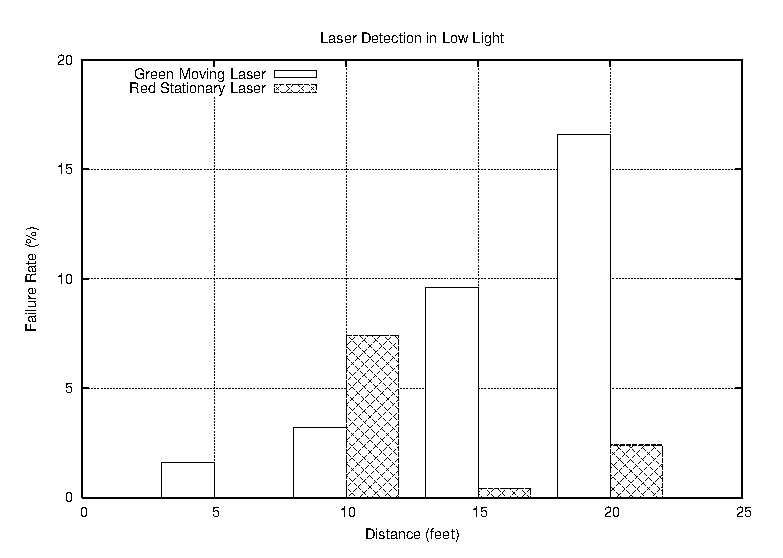
\includegraphics[width=0.8\linewidth]{laser_low.eps}
\end{center}
   \caption{Laser detection in Low Light.}
\label{fig:laser_low}
\label{fig:long}
\label{fig:onecol}
\end{figure}

\begin{figure}[t]
\begin{center}
  \includegraphics[width=0.8\linewidth]{laser_high.eps}
\end{center}
   \caption{Laser detection in High Light.}
\label{fig:laser_high}
\label{fig:long}
\label{fig:onecol}
\end{figure}

It is important to note that these tests demonstrate false negatives, or failure of our implementation to detect a laser point when it appeared in the camera view.  These tests are not able to show the false postive rates, or when spurious/outlier pixels are incorrected detected as a genuine laser point pixel.  To accurately detect or measure false positives is particularly difficult as they are manifested as imprecise detections.  The most obvious example is when a laser point is detected when there is actually none in camera view.  In our testing, we noticed that in certain situations, the detected center of the red laser was offset some pixels from the actual center.  This is an example of jitter, caused by some false positive detections.  We were unable to quantify the rates of false positives because it would require a human to examime each frame of video to check for jitter.  This would be a tedious process and requires a large investment of time, which we do not have.

\subsection{Distance Estimation}

\begin{figure}[t]
\begin{center}
  \includegraphics[width=0.8\linewidth]{distance_estimation.eps}
\end{center}
   \caption{Distance estimation.}
\label{fig:distance_estimation}
\label{fig:long}
\label{fig:onecol}
\end{figure}

The results for the distance estimation are located in ~\ref{fig:distance_estimation}.

The distance estimation was not implemented into the turret aim logic due to the low accuracy at distances over eight feet. One of the problems was that the distance estimation accuracy is directly related to how far the distance laser is mounted away from the optical axis.  

\subsection{Turret Accuracy}


\section{Discussion and Conclusion}


\section{Future Work}

In order for the algorithm to work, proper threshold values must be chosen for the Hue and Value images.  This requires manual calibration by the user.  Different values for thresholds must be experimented with until a satisfactorily thresholded final image is generated - one that only shows the laser point.  Though not a priority, it may be possible to greatly reduce manual calibration by allowing the computer to sample incoming images with incrementally different threshold values.  Once an image with a single small cluster of white pixels is found, the automatic calibration would be complete.

Another improvement could be made using differing combinations of HSV values, or perhaps even one using a different color space altogether.  For example, though our initial tests show that Hue and Value channels ANDed together is an effective approach, perhaps in a different lighting situation, a combination of Hue and Saturation channels would be more useful.  Ultimately, these combinations would require a great deal more testing in different environments than time constraints will allow.  Because of these time constraints, we have only implemented a manual approach to laser light detection.  However, due to testing, we have discovered useful initialization values.  These values can naturally be adjusted by the user during run-time.

As future work, a complete hardware design would be a high priority.  The NXT hardware, along with the lego construction, while sufficient for our testing purposes, is not sturdy or robust enough for high-speed response to laser detection.  The current implementation takes a considerable amount of time to aim and repositioning before a shot is fired.  In a real-world scenario, turret adjustment time should be measured in milliseconds, not seconds or even minutes.  For this high speed setup, we would need industrial-quality servos, sturdy construction materials, possibly metal, and possibly customized controller electronics.

The camera was also a source of error.  Naturally, for the best possible detection, the best possible camera must be used.  A professional camera with a high frame rate (30+ fps) and resolution, along with stable performance and high speed, uncompressed data transfer would be extremely useful.

The software speed may be improved by switching from Python to C/C++.  With a compiled language, more filtering features may be implemented with far less reduction in speed, such as the naive lonely pixel removal function described earlier.  Automatic calibration is another feature worth researching in the future.

{\small
\bibliographystyle{ieee}
\bibliography{egbib}
}

\end{document}
